\documentclass{article}
\usepackage[T1]{fontenc}
\usepackage[utf8]{inputenc}
\usepackage{lmodern}
\usepackage[polish,shorthands=off]{babel}
\usepackage{graphicx}
\usepackage{siunitx}
\usepackage{multirow}
\usepackage{longtable}
\usepackage{hyperref}
\usepackage[all]{hypcap}
\usepackage{float}
\usepackage{enumitem}
\usepackage{tikz}
\usetikzlibrary{positioning}
\usepackage{amsmath}
\usepackage[linesnumbered,ruled]{algorithm2e}

\usepackage{framed}
\definecolor{shadecolor}{gray}{0.88}

\title{Sprawozdanie Algorytmy Dyskretne\\Lista 4}
\author{Jakub Kowal}
\date{}
\begin{document}
\maketitle

\section{Algorytm Edmondsa-Karpa}
\subsection{Implementacja}
Moja implementacja algorytmu Edmondsa-Karpa działa w następujący sposób:
\SetAlgorithmName{Edmonds-Karp}{}{}
\begin{algorithm}[H]
    \SetKwInOut{Input}{Input}
    \SetKwInOut{Output}{Output}

    \Input{źródło s, cel t}
    \Output{Maksymalny możliwy przepływ}
    \While{True (faktycznie to dopóki jest ścieżka powiększająca z s do t)}{
        queue.push(s)\;
        //Szukanie ścieżki poprzez BFS (zwraca minimalny łuk residualny)
        \eIf{Nie ma ścieżki powiększającej}{
            break;
        }
        {
            //Przejdź znalezioną ścieżką powiekszającą od końca (t) i powiększaj o znaleziony pathFlow
        }

    }
    return maxFlow;
      \caption{}
\end{algorithm}
\subsection{Złożoność}

\section{Algorytm Dinica}
\SetAlgorithmName{Dinic}{}{}
\begin{algorithm}[H]
    \SetKwInOut{Input}{Input}
    \SetKwInOut{Output}{Output}

    \Input{źródło s, cel t}
    \Output{Maksymalny możliwy przepływ}
    \While{True (faktycznie to dopóki jest ścieżka powiększająca z s do t)}{
        queue.push(s)\;
        //Szukanie ścieżki poprzez BFS (zwraca minimalny łuk residualny)
        \eIf{Nie ma ścieżki powiększającej}{
            break;
        }
        {
            //Przejdź znalezioną ścieżką powiekszającą od końca (t) i powiększaj o znaleziony pathFlow
        }

    }
    return maxFlow;
      \caption{}
\end{algorithm}
\subsection{Implementacja}
\subsection{Złożoność}

\section{Zapisywanie do modeli LP}
\subsection{Implementacja}
Klasa FlowNetwork zwyczajnie zapisuje do pliku .jl najpierw wstęp potrzebny do modelu. Potem zapisuje ograniczenia przepływu wszystkich krawędzi (domyślnie jest 0) jako macierz kwadratową \textit{G}. Jako zmienną tworzy macierz kwadratową \textit{f} z ograniczeniami zapisanymi wcześniej w \textit{G}. Następnie zapewnia ograniczeniami, że węzły inne niż \textit{{s,t}} będą przyjmowały taki sam przepływ jaki przekazują dalej. Ostatecznie maksymalizujemy sumę przepływów wychodzących z pierwszego węzła, czyli naszego \textit{s}.

\section{Zadanie Hiperkostka}
\subsection{Opis zadania}
\subsection{Wyniki}
Wyniki są średnimi wartościami 25 powtórzeń.
\begin{figure}[H]
    \caption{Wykres czasu względem k}
    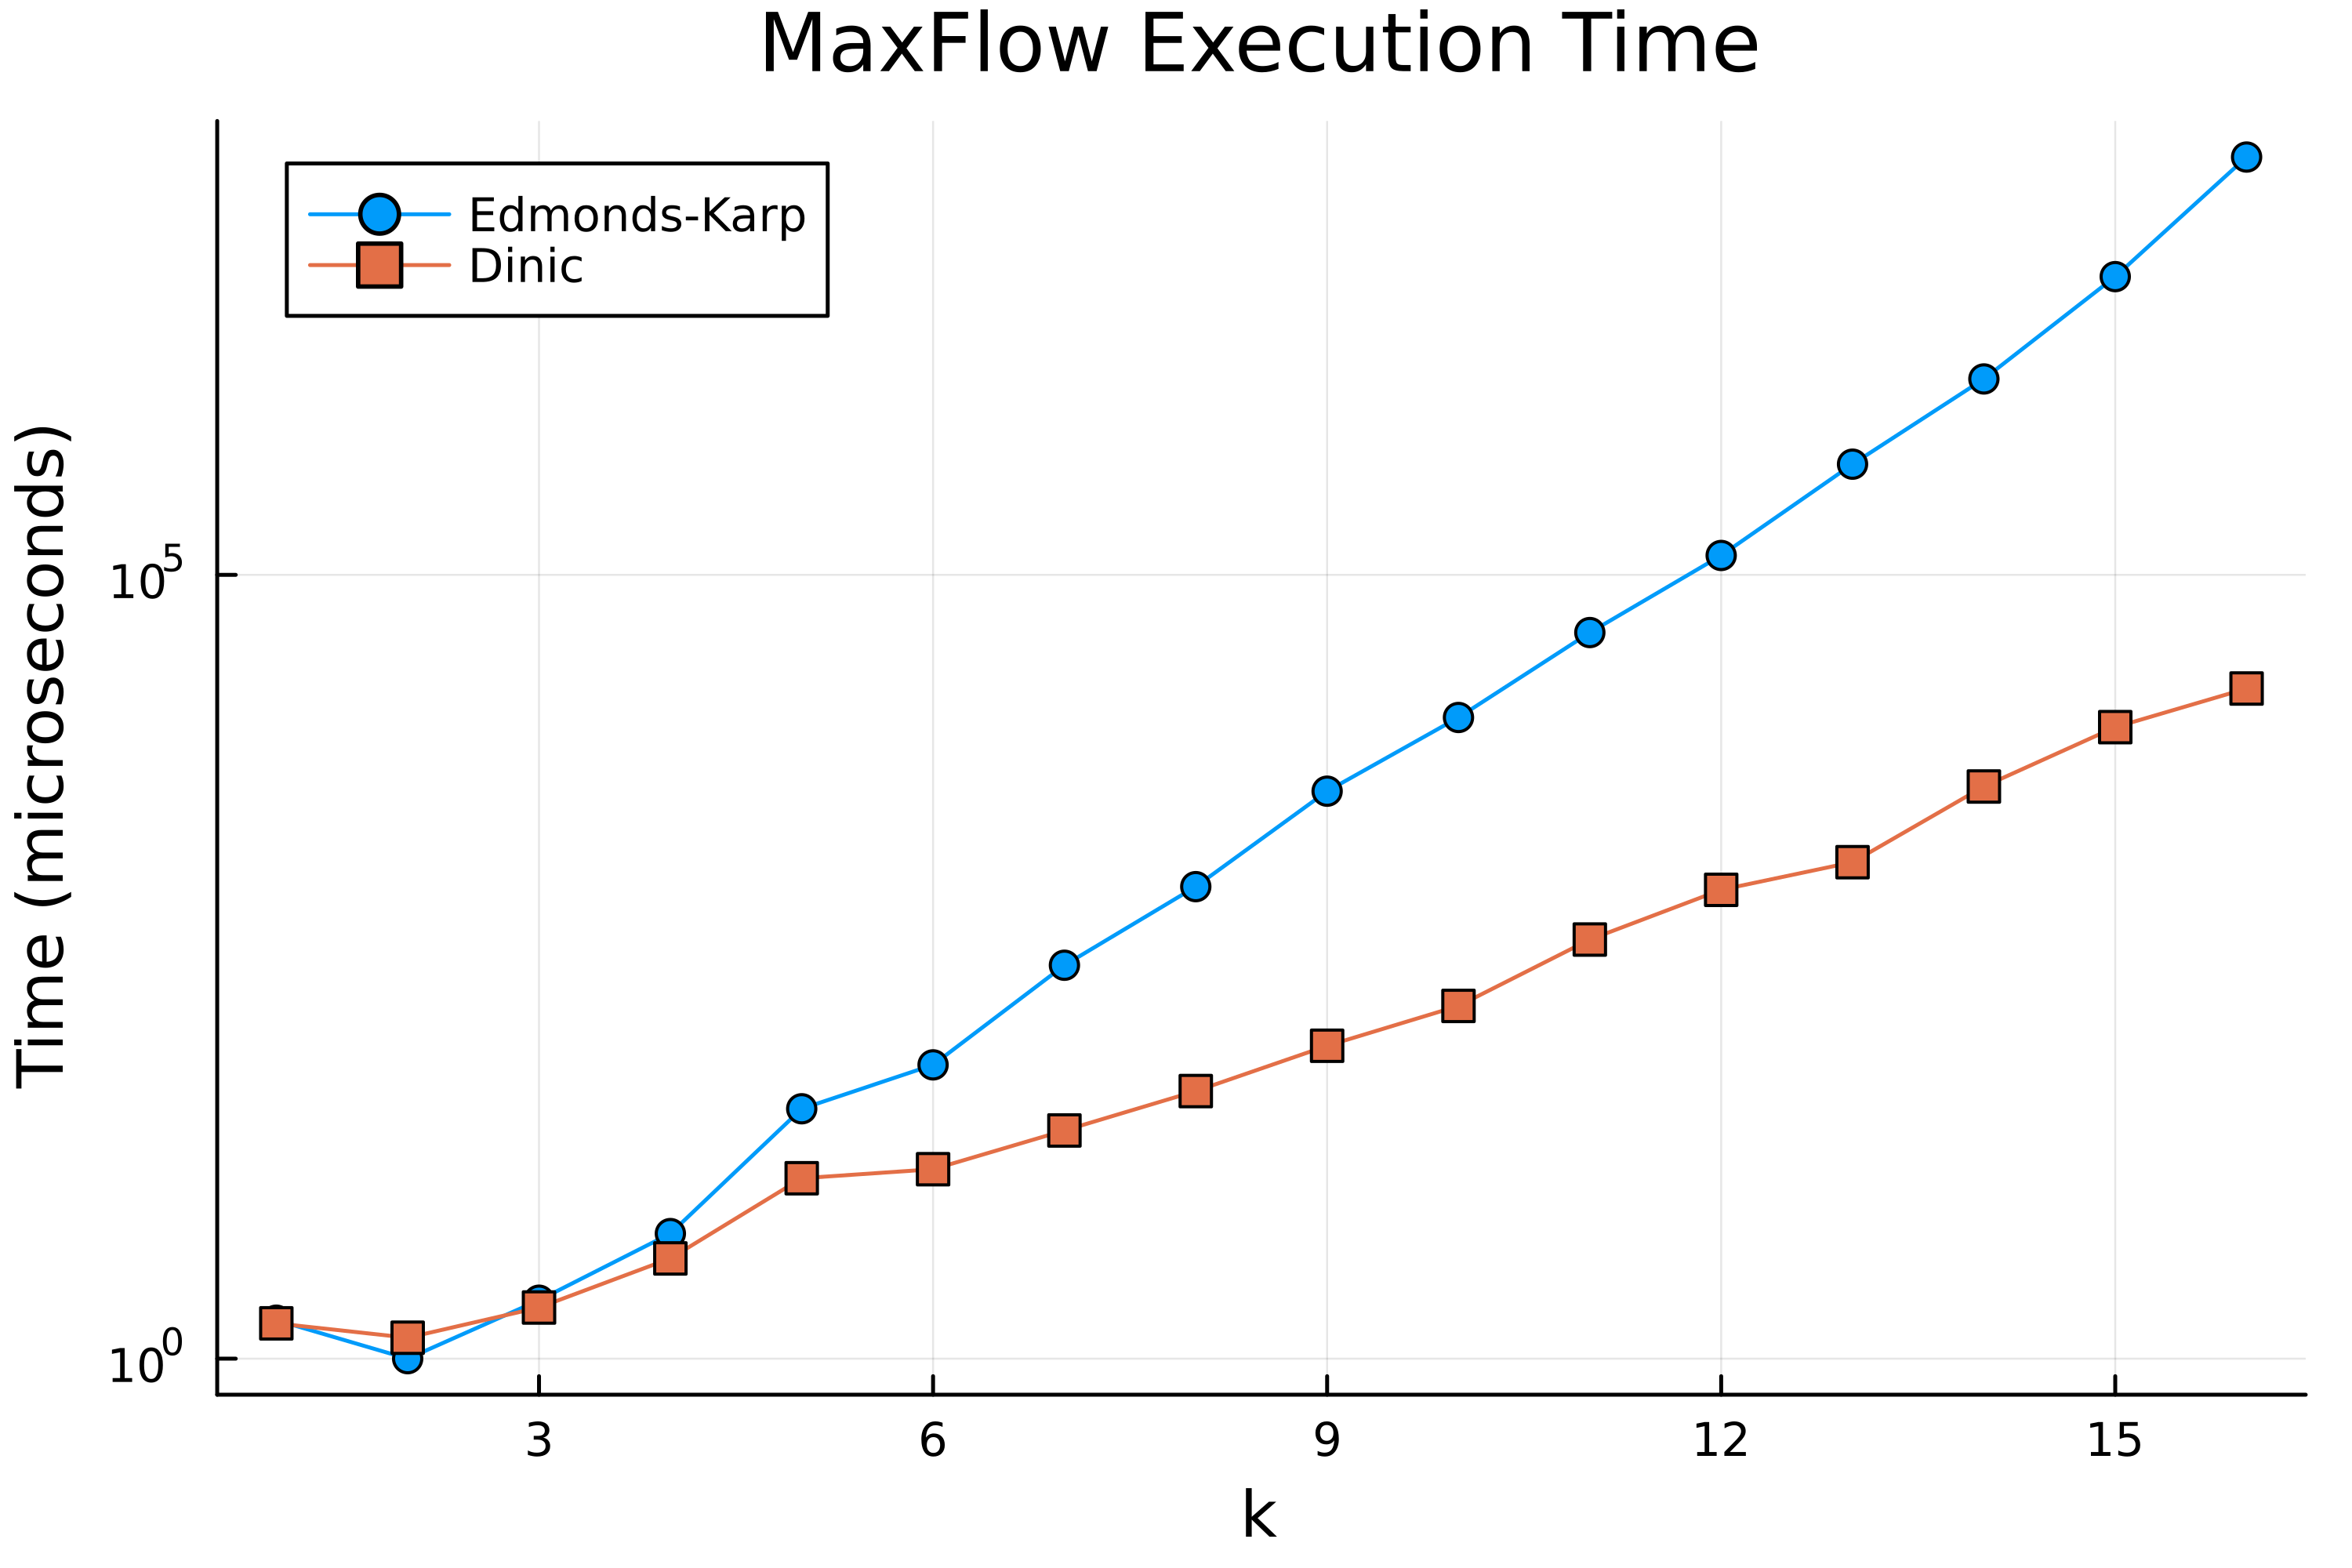
\includegraphics[width=35em]{../plots/flow_time.png}
    \label{fig:Z1_times}
\end{figure}
\begin{figure}[H]
    \caption{Wykres ilości ścieżek powiększających względem k}
    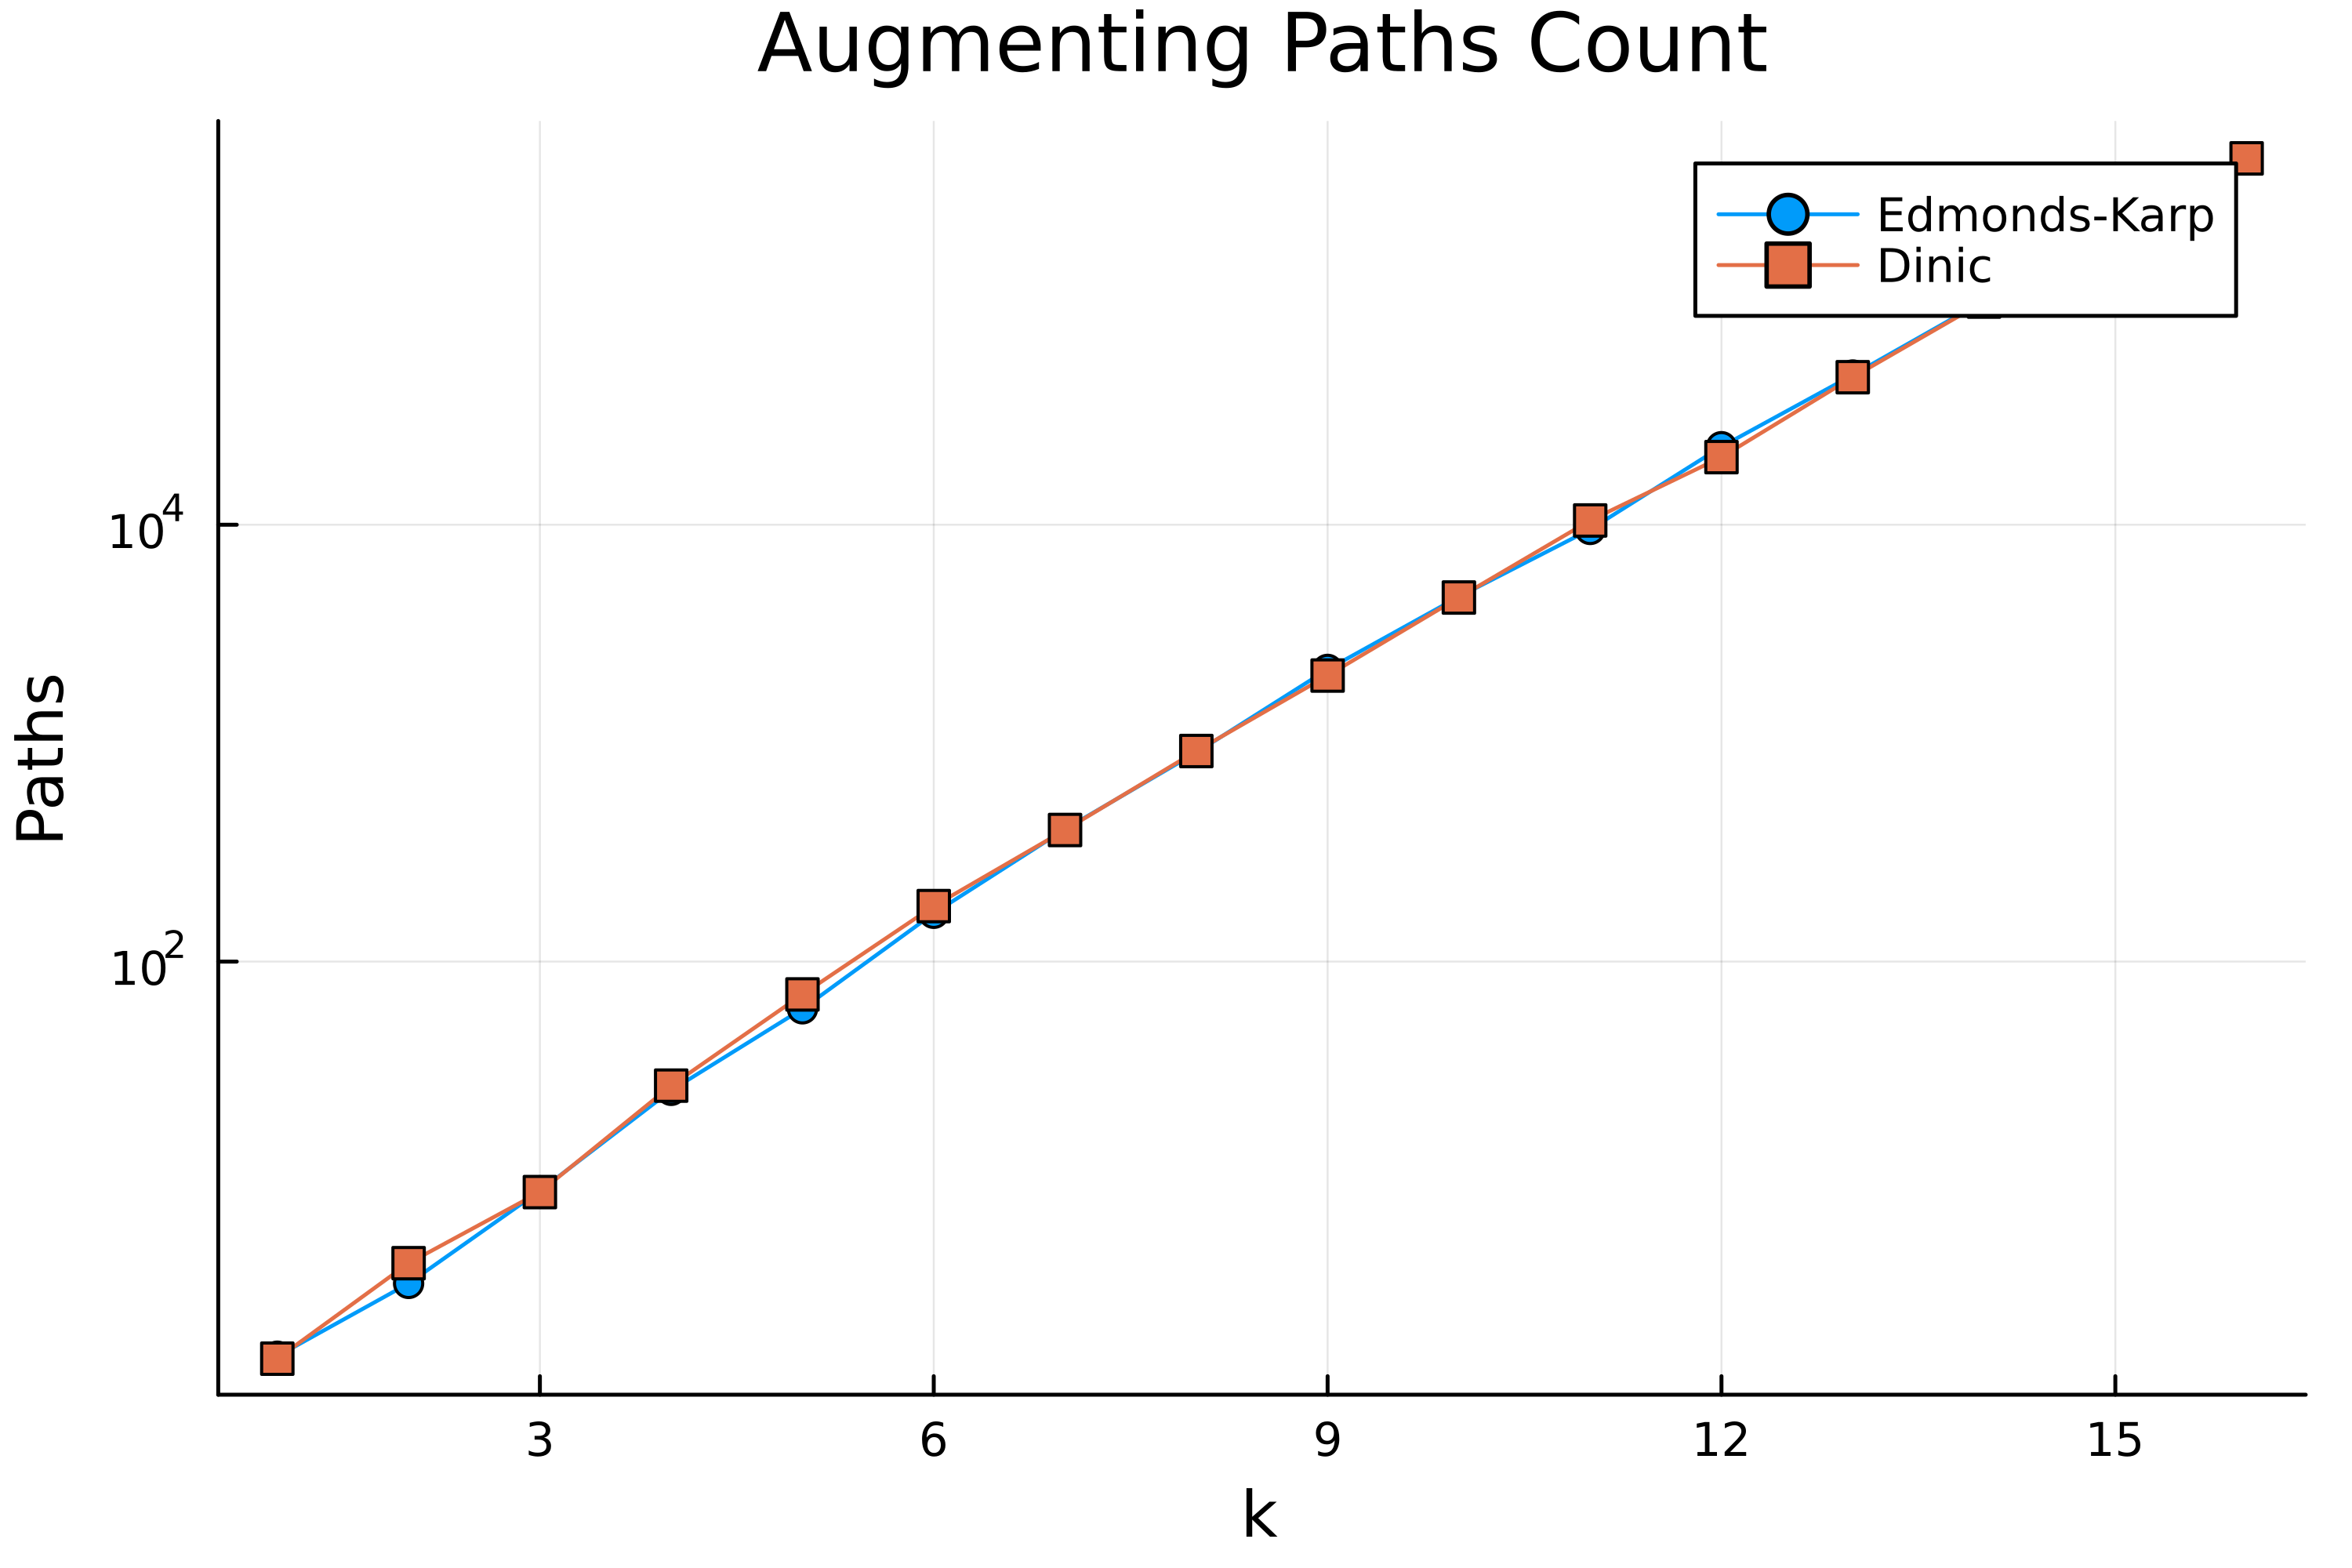
\includegraphics[width=35em]{../plots/flow_count.png}
    \label{fig:Z1_flows}
\end{figure}
\begin{figure}[H]
    \caption{Wykres maksymalnego przepływu względem k}
    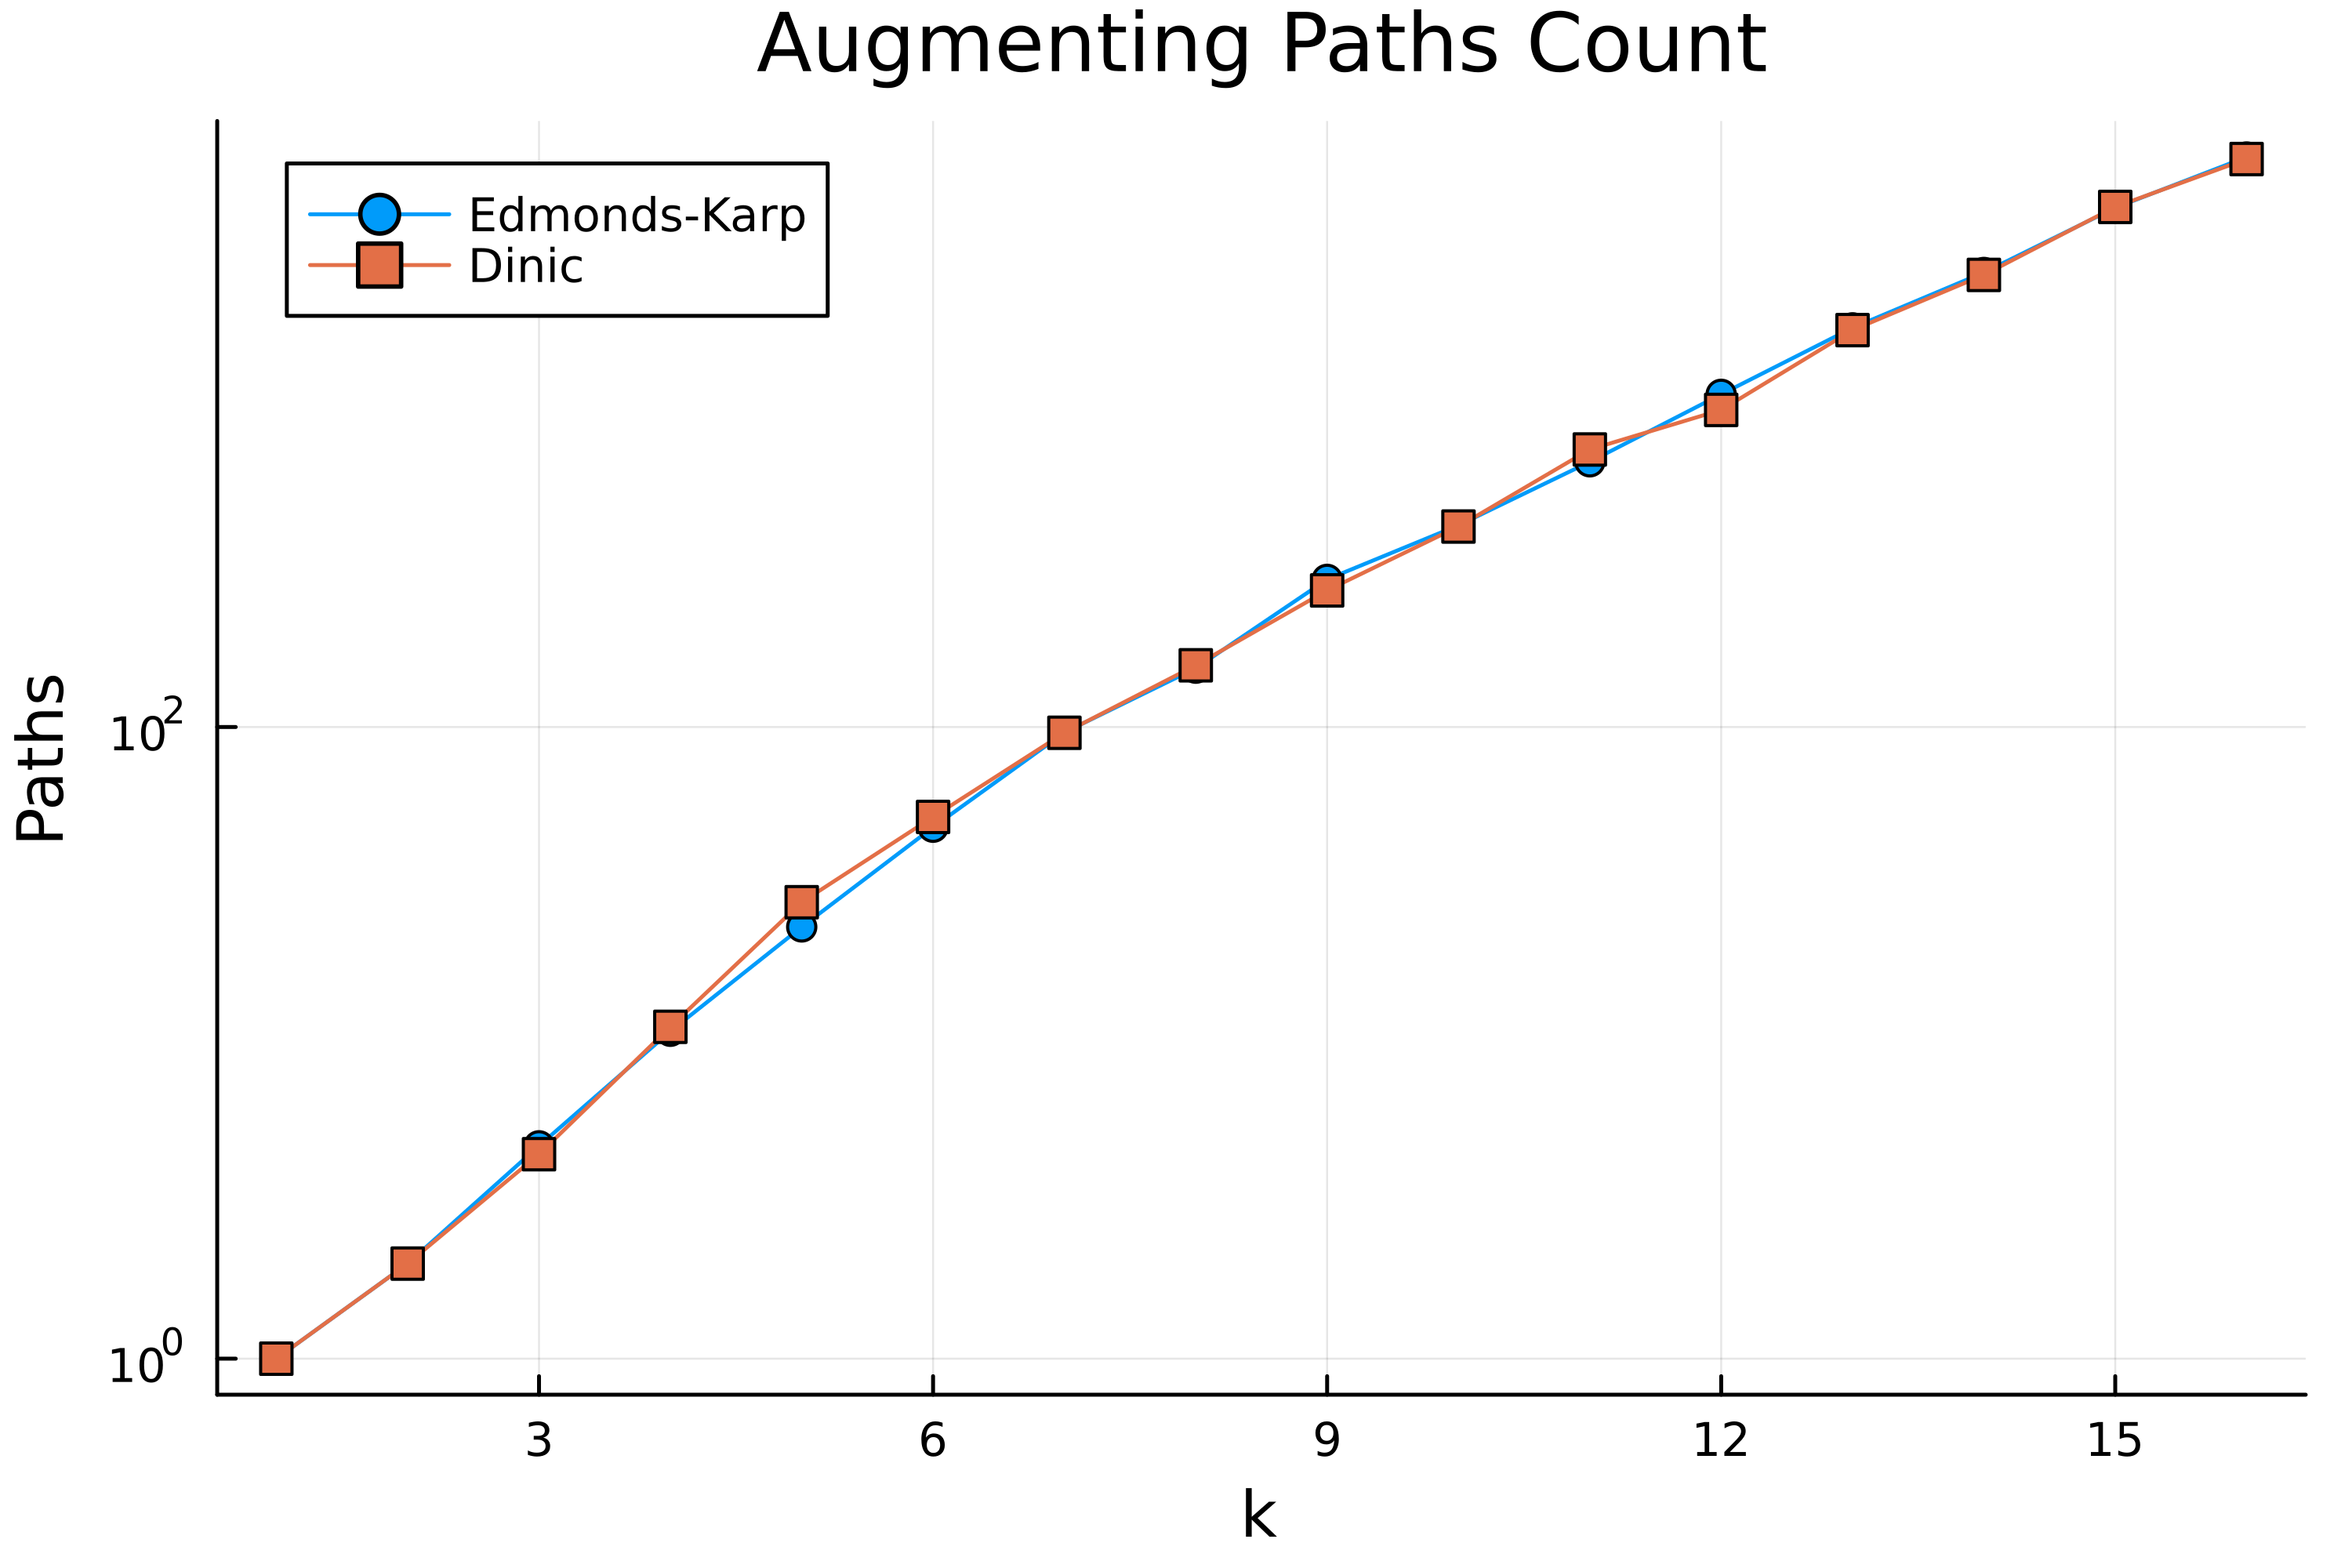
\includegraphics[width=35em]{../plots/flow_paths.png}
    \label{fig:Z1_paths}
\end{figure}

\subsection{Wnioski}
Jak widać na \hyperref[fig:Z1_flows]{wykresie maksymalnego przepływu} oraz \hyperref[fig:Z1_paths]{wykresie ścieżek powiększających} oba algorytmy zwracały niesamowicie zbliżone wyniki. Różnicę natomiast widać na \hyperref[fig:Z1_times]{wykresie czasu}, jaki te algorytmy potrzebowały na rozwiązanie problemu. Oba algorytmy bardzo dobrze poradziły sobie z zadaniem, ale wyraźnie widać przewagę algorytmu Dinica. 

\section{Zadanie Maksymalne Skojarzenia}
\subsection{Opis zadania}
Prowizoryczna wizualizacja grafu:
\begin{center}
    \begin{tikzpicture}[
    roundnode/.style={circle, draw=black, fill=white, thick, minimum size=9mm},
    emptynode/.style={circle, draw=white, fill=white, thick, minimum size=9mm}
    ]
    %Left nodes
    \node[roundnode]        (left_first)                              {1};
    \node[roundnode]        (left_second)           [below=of left_first] {2};
    \node[emptynode]        (left_middle)           [below=of left_second] {\dots};
    \node[roundnode]        (left_second_to_last)   [below=of left_middle] {n-1};
    \node[roundnode]        (left_last)             [below=of left_second_to_last] {n};
    \node[roundnode]        (source)                [left=of left_middle] {s};

    %Dystans
    \node[emptynode]        (distance)              [right=of left_first]   {};

    %Right nodes
    \node[roundnode]        (right_first)            [right=of distance]                {1};
    \node[roundnode]        (right_second)           [below=of right_first] {2};
    \node[emptynode]        (right_middle)           [below=of right_second] {\dots};
    \node[roundnode]        (right_second_to_last)   [below=of right_middle] {n-1};
    \node[roundnode]        (right_last)             [below=of right_second_to_last] {n};
    \node[roundnode]        (sink)                   [right=of right_middle] {s};

    %Lines
    \draw[->]   (source) -- (left_first);
    \draw[->]   (source) -- (left_second);
    \draw[->]   (source) -- (left_second_to_last);
    \draw[->]   (source) -- (left_last);

    \draw[dashed,->]    (left_first) -- (right_first);
    \draw[dashed,->]    (left_first) -- (right_second);
    \draw[dashed,->]    (left_first) -- (right_second_to_last);
    \draw[dashed,->]    (left_first) -- (right_last);

    \draw[dashed,->]    (left_second) -- (right_first);
    \draw[dashed,->]    (left_second) -- (right_second);
    \draw[dashed,->]    (left_second) -- (right_second_to_last);
    \draw[dashed,->]    (left_second) -- (right_last);

    % \draw[dashed,->]    (left_second_to_last) -- (right_first);
    % \draw[dashed,->]    (left_second_to_last) -- (right_second);
    % \draw[dashed,->]    (left_second_to_last) -- (right_second_to_last);
    % \draw[dashed,->]    (left_second_to_last) -- (right_last);

    % \draw[dashed,->]    (left_last) -- (right_first);
    % \draw[dashed,->]    (left_last) -- (right_second);
    % \draw[dashed,->]    (left_last) -- (right_second_to_last);
    % \draw[dashed,->]    (left_last) -- (right_last);

    \draw[->]   (right_first) -- (sink);
    \draw[->]   (right_second) -- (sink);
    \draw[->]   (right_second_to_last) -- (sink);
    \draw[->]   (right_last) -- (sink);

    \end{tikzpicture}
\end{center}

\subsection{Wyniki}

\end{document}